\documentclass{sigchi}

% Use this command to override the default ACM copyright statement
% (e.g. for preprints).  Consult the conference website for the
% camera-ready copyright statement.

%% EXAMPLE BEGIN -- HOW TO OVERRIDE THE DEFAULT COPYRIGHT STRIP -- (July 22, 2013 - Paul Baumann)
% \toappear{Permission to make digital or hard copies of all or part of this work for personal or classroom use is      granted without fee provided that copies are not made or distributed for profit or commercial advantage and that copies bear this notice and the full citation on the first page. Copyrights for components of this work owned by others than ACM must be honored. Abstracting with credit is permitted. To copy otherwise, or republish, to post on servers or to redistribute to lists, requires prior specific permission and/or a fee. Request permissions from permissions@acm.org. \\
% {\emph{CHI'14}}, April 26--May 1, 2014, Toronto, Canada. \\
% Copyright \copyright~2014 ACM ISBN/14/04...\$15.00. \\
% DOI string from ACM form confirmation}
%% EXAMPLE END -- HOW TO OVERRIDE THE DEFAULT COPYRIGHT STRIP -- (July 22, 2013 - Paul Baumann)

% Arabic page numbers for submission.  Remove this line to eliminate
% page numbers for the camera ready copy
% \pagenumbering{arabic}

% Load basic packages
\usepackage{balance}  % to better equalize the last page
\usepackage{graphics} % for EPS, load graphicx instead 
\usepackage[T1]{fontenc}
\usepackage{txfonts}
\usepackage{mathptmx}
\usepackage[pdftex]{hyperref}
\usepackage{color}
\usepackage{booktabs}
\usepackage{textcomp}
% Some optional stuff you might like/need.
\usepackage{microtype} % Improved Tracking and Kerning
% \usepackage[all]{hypcap}  % Fixes bug in hyperref caption linking
\usepackage{ccicons}  % Cite your images correctly!
% \usepackage[utf8]{inputenc} % for a UTF8 editor only
\usepackage{glossaries}
\usepackage{enumitem}
\usepackage{subcaption}

% If you want to use todo notes, marginpars etc. during creation of your draft document, you
% have to enable the "chi_draft" option for the document class. To do this, change the very first
% line to: "\documentclass[chi_draft]{sigchi}". You can then place todo notes by using the "\todo{...}"
% command. Make sure to disable the draft option again before submitting your final document.
\usepackage{todonotes}

% Paper metadata (use plain text, for PDF inclusion and later
% re-using, if desired).  Use \emtpyauthor when submitting for review
% so you remain anonymous.
\def\plaintitle{A Comparison of Nelder-Mead and Bayesian Optimization\\
for Mixed-Initiative Exploration of Machine Parameters}
\def\plainauthor{Andrew Head}
\def\emptyauthor{}
% \def\plainkeywords{Authors' choice; of terms; separated; by
%   semicolons; include commas, within terms only; required.}
\def\plainkeywords{mixed-initiative interaction; user preference modeling; numerical optimization; fabrication;}
% \def\plaingeneralterms{Documentation, Standardization}
\def\plaingeneralterms{mixed-initiative interaction; fabrication hardware; making; novices}

% llt: Define a global style for URLs, rather that the default one
\makeatletter
\def\url@leostyle{%
  \@ifundefined{selectfont}{
    \def\UrlFont{\sf}
  }{
    \def\UrlFont{\small\bf\ttfamily}
  }}
\makeatother

% llt: Define a global style for URLs, rather that the default one
\makeatletter
\def\url@leostyle{%
  \@ifundefined{selectfont}{
    \def\UrlFont{\sf}
  }{
    \def\UrlFont{\small\bf\ttfamily}
  }}
\makeatother
\urlstyle{leo}

% To make various LaTeX processors do the right thing with page size.
\def\pprw{8.5in}
\def\pprh{11in}
\special{papersize=\pprw,\pprh}
\setlength{\paperwidth}{\pprw}
\setlength{\paperheight}{\pprh}
\setlength{\pdfpagewidth}{\pprw}
\setlength{\pdfpageheight}{\pprh}

% Make sure hyperref comes last of your loaded packages, to give it a
% fighting chance of not being over-written, since its job is to
% redefine many LaTeX commands.
\definecolor{linkColor}{RGB}{6,125,233}
\hypersetup{%
  pdftitle={\plaintitle},
% Use \plainauthor for final version.
%  pdfauthor={\plainauthor},
  pdfauthor={\emptyauthor},
  pdfkeywords={\plainkeywords},
  bookmarksnumbered,
  pdfstartview={FitH},
  colorlinks,
  citecolor=black,
  filecolor=black,
  linkcolor=black,
  urlcolor=linkColor,
  breaklinks=true,
  hypertexnames=false
}

% create a shortcut to typeset table headings
% \newcommand\tabhead[1]{\small\textbf{#1}}

% End of preamble. Here it comes the document.
\begin{document}

\title{\plaintitle}

\numberofauthors{1}
\author{%
  \alignauthor{Andrew Head\\
    \affaddr{UC Berkeley}\\
    \affaddr{Berkeley, CA, USA}\\
    \email{andrewhead@eecs.berkeley.edu}}\\
  \if 0
  \alignauthor{Leave Authors Anonymous\\
    \affaddr{for Submission}\\
    \affaddr{City, Country}\\
    \email{e-mail address}}\\
  \alignauthor{Leave Authors Anonymous\\
    \affaddr{for Submission}\\
    \affaddr{City, Country}\\
    \email{e-mail address}}\\
  \fi
}

\maketitle

\begin{abstract}
People frequently work with machines to produce artifacts.
While they know their end goal, it can be difficult to express it with the parameters the machine makes available.
This paper studies algorithms to help users explore a space of unfamiliar machine parameters in pursuit of a known goal.
It aims to understand the performance of two algorithms in terms of speed of convergence to the human's goal, and the human's trust.
The algorithms are Nelder-Mead and a variant of Bayesian optimization.
I build for front-end for each one where a user provides comparison-based ratings of examples to guide the algorithm.
With a 28-participant Mechanical Turk study, I compare the algorithms.
While a Bayesian Optimization algorithm appeared more random to participants, they felt that it better achieved the goal.
Nelder-Mead appeared to get better over time to participants, it seemed more likely to get stuck.
The study provides justification and criteria for a systematic evaluation of the affordances, human perceptions, and performance of algorithms for exploring parameter spaces.
\end{abstract}


% System names
\newglossaryentry{systemname}
{%
    name=FabExample,
    description={A system for mixed-initiative exploration of a fabrication machine's parameter space.}
}

% Revision Macros
\newcommand{\andrew}[1]{{\color{red}\textbf{AH\@: #1}\normalfont}}
\newcommand{\bjoern}[1]{{\color{blue}\textbf{BH\@: #1}\normalfont}}
\newcommand{\shortchange}[1]{{\color{OliveGreen}\textbf{#1}\normalfont}}
% \newcommand{\shortchange}[1]{{#1}}
\newenvironment{changes}{\shortchange\bgroup}{\egroup}


%\category{H.5.m.}{Information Interfaces and Presentation
%  (e.g. HCI)}{Miscellaneous} \category{See
%  \url{http://acm.org/about/class/1998/} for the full list of ACM
%  classifiers. This section is required.}{}{}
\category{H.5.2.}{User Interfaces}{Training, help, and documentation.  Interaction Styles.}
% \category{H.5.2.}{User Interfaces}{Interaction styles}

\keywords{\plainkeywords}

\section{Introduction}

\begin{figure}
  \centering
  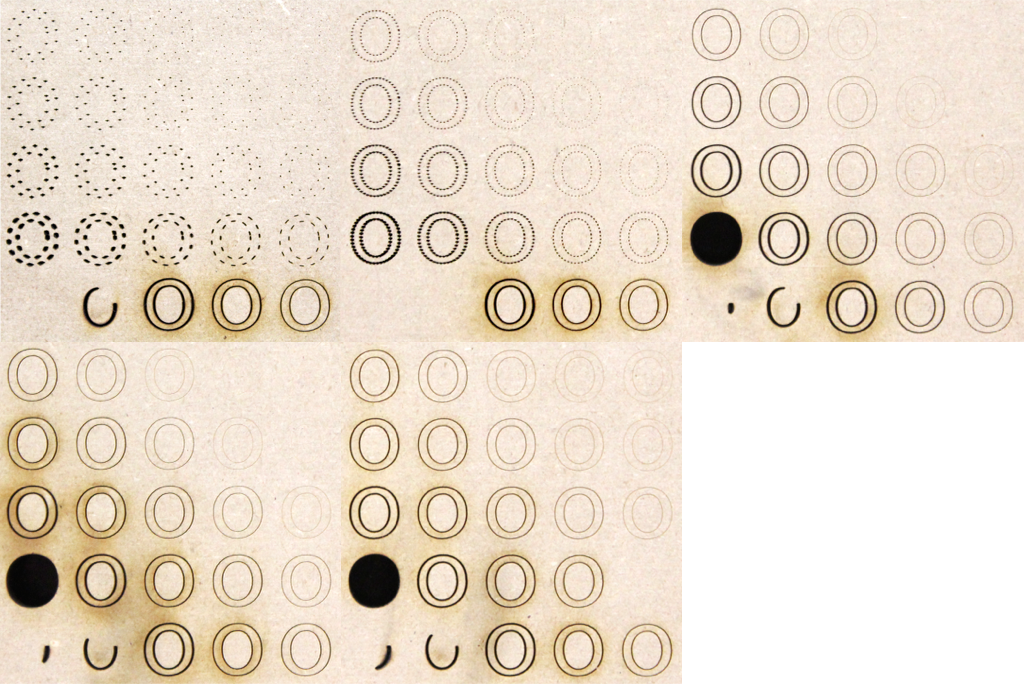
\includegraphics[width=0.4\textwidth]{figures/engravings}
  \caption{%
    A user of the laser cutter has to manipulate the laser's parameters to get the desired appearance.
    Black holes are when the laser passes completely through the material---
    the center is cut out and falls through.
  }\label{fig:rasters}
\end{figure}

\andrew{Make sure to tie this into what my contributions are to our class and what they should take away.}

As you enter the Invention Lab, Berkeley's student hackerspace, you quickly notice that learning to work with fabrication machines is hard.
Scorched cardboard sits atop the scrap pile from laser-cut materials that caught fire.
Failed 3D prints line the foyer walls, deformed from thin supports and improper orientations.
Consider what it takes to configure a laser cutter to ``raster'' images onto workpieces:
four different parameters control the depth, speed, and fidelity of the image etched into the material.
Improper values cause the image to appear only faintly, or melt the material (see Figure~\ref{fig:rasters}).

This research pursues a vision for fabrication machines that help users learn how to operate them.
My key insight is that a fabrication machine can be equipped with an active learning algorithm to enable mixed initiative exploration of a parameter space.
I implement this for a laser cutter and a maker rastering images.
My intended contributions are:
\begin{enumerate}
\item A catalog of user problems realizing design intent with laser cutters
\item Application of active learning to discovering an ideal fabrication machine configuration
\item A comparison of mixed initiative parameter exploration with self-led approaches
\end{enumerate}

To understand frequency, severity, and types of errors makers encounter with laser cutters, I will interview a small number of student members of the Invention Lab.

I will implement an active learning algorithm~\cite{settles_active_2010} to guide a machine, with a user's help, to some subjective ideal configuration for rastering an image.
Each configuration will comprise laser power, speed, frequency, and resolution.
The algorithm will suggest configurations and demonstrate them by rastering an image.
The algorithm will collect a user's rating of raster quality.
As the learned model will predict an continuous value, I will draw from past work for actively learning continuous-value models (e.g.~\cite{sugiyama_active_2008}).
% Currently, I suspect that a Gaussian kernel function or a quadratic curve will best express a user's perception of the quality of a configuration in actualizing their design.

To understand the trade-offs of this method of mixed initiative parameter space exploration, I will run a usability study.
Participants will be asked to recover a configuration for rastering an image that matches an exemplar I provide.
The method of parameter exploration will be varied:
in one condition, participants explore configurations on their own.
In the other, participants explore the configuration space prompted by the examples provided by the active learning algorithm.
Among other metrics, I will measure the total number of configurations tested, and Likert scale and open-ended feedback on perceptions of the experience.

The usability study will use a Universal Laser Systems VLS3.50 machine.
I have received clearance to work with this equipment.
Given the limited time available for the hardware, the proposed usability study will likely include around 4--6 participants.


\section{Related Work}

\subsection{Optimizing Black Box Functions}

We draw upon a rich history of related work on optimization for black box functions.
This can trace its origins back to optimal experiment design~\cite{box}.
The intent of optimal experiment design is to (quote from Box \& Draper).

Related techniques for methods for numerically determining an optimum include:
\begin{itemize}
  \item Nelder-Mead method~\cite{nelder}
  \item Evolutionary strategies (e.g., covariance matrix adaptation (CMA-ES))~\cite{cma}
  \item Bayesian optimization~\cite{brochu_tutorial_2010}
  \item Gaussian processes~\cite{gaussian}
  \item Response Surface Modeling~\cite{box}
  \item Reinforcement learning~\cite{reinforcement}
\end{itemize}

We draw upon the principles for successful determination models from the generic techniques from the body of literature on active learning~\cite{al} and multi-arm bandit problems~\cite{multi-armed}.
An overarching theme from this body of work is ``exploration'' vs.\ ``exploitation''.
This means that a large enough portion of the function's domain is covered to be reasonably certain that optima found are global, not local;
at the same time, the algorithm does not spend too long exploring regions that are not likely to contain the global optimum.

Philosophically, this work aims to lessen the effort to train a machine to learn a human's model of ideal behavior.
In this aim, it is similar to past work on robotic ``clicker training''~\cite{clicker_1}~\cite{clicker_2}.
Clicker training aims to teach robots complex behavior with a single binary input channel that can reward partial behaviors until a robot builds up the full behavior.
This can be considered a simple version of reinforcement learning~\cite{reinforcement}, where a human judge offers rewards to a robot so that it can learn an ideal policy of how to act when it's in a certain state.

One domain highly related to our domain of interest is that of user preference modeling.
For an example of a problem framing of Bayesian optimization for user preference modeling, see~\cite{brochu_tutorial_2010}.

\subsection{Assistive Fabrication Devices}

A growing body of recent work has focused on improving makers' ability to express their intentions with fabrication machines.
Relevant papers include \ldots


\section{Algorithms}

I implement two algorithms that enable the discovery of user preferences.
Here, I provide a brief introduction to each of the algorithms.
I describe the steps taken to modify the algorithms to accept comparisons as input to drive optimization.
I also describe how bounds are enforced for each one, the initial points of each algorithm, and the hyperparameters used.

The input space for each algorithm was discretized, with a log-scale for each of three dimensions: the laser cutter's settings for power, speed, and PPI\@.
Power and speed ranged from 1--100\%.
Possible values for these two dimensions were:
$\left[1\%, 3\%, 10\%, 32\%, 100\%\right]$.
PPI ranged within 10--1000, with possible values:
$\left[10, 32, 100, 316, 1000\right]$.
In the space below, configurations are described as three-tuples:
$\left(Power, Speed, PPI\right)$.
For a discussion of how each of these parameters impact the laser cutter's operation, see~\cite{versalaser_2010}.

\subsection{Nelder-Mead Optimization}

Nelder-Mead is an optimization method that iteratively moves vertices of a simplex towards the best-rated vertex~\cite{nelder_simplex_1965}.
For reflection, expansion, and contraction, we chose coefficients observed as the best in the original Nelder-Mead work~\cite{nelder_simplex_1965}:
$\alpha=1$,
$\gamma=2$,
$\beta=-1/2$,
and a reduction coefficient of 1/2.

To perform Nelder-Mead optimization, the algorithm doesn't need to know an exact evaluation for each vertex.
It only needs to know which is the best, second-to-worst, and worst points out of each set of vertices.

Initially, the vertices were:
(1\%, 1\%, 10),
(1\%, 1\%, 1000),
(1\%, 100\%, 10),
(100\%, 1\%, 10),
These points were chosen for two reasons.
First, at least four points are needed to migrate to all possible points in 3D space.
(With any three points, all three and their centroid would reside on a single plane.
Any reflection, expansion, contraction computed as a transformation of a difference vector on that plane yields another point on that plane.)
Second, it was clear from viewing this collection of points that extremes of appearance were shown.
For example, one image consisted of very sparse dots, another of very light lines, and another showed dark, thick lines.

\subsection{Bayesian Optimization}

Each iteration of Bayesian optimization comprises two steps~\cite{brochu_tutorial_2010}:
fitting a Gaussian process to the data seen so far, and sampling a new value likely to maximize the unknown cost function.
Typically, selection of the sample in the second step is performed by maximizing \emph{expected improvement}.
Based on the work by Brochu et al.~\cite{brochu_tutorial_2010}, I express this as combination of two terms for exploration and exploitation:
\begin{equation}
EI (x) = (\mu(x) - f (x^+)) \Phi(Z) + \sigma(x) \phi(Z)
\end{equation}
where $Z = \frac{\mu(x) - f(x^+)}{\sigma(x)}$ is in the domain of a normal distribution, representing the probability of improvement at $x$;
$\mu(x)$ is the predicted value of a new input $x$;
$f(x^+)$ is highest value seen so far;
$\sigma(x)$ is the standard deviation at $x$;
$\phi(Z)$ and $\Phi(Z)$ are the probability and cumulative density functions for $Z$.

Brochu et al.~\cite{brochu_tutorial_2010}~\cite{brochu_active_2008} propose a variant on Bayesian optimization that takes comparisons between sampled points as inputs.
I implement this algorithm for this study.
I used a squared exponential kernel with $\sigma = 0.25$.
In performing Newton-Rhapson optimization according to Brochu et al.'s formulation, $\sigma_{noise}$ was set to 10, and ten iterations were performed to optimize the Gaussian process.
These parameters were chosen by trial and error, observing what appeared to enable convergence in the target 3D input space for this study.
Caching and limited iterations were implemented to ensure the algorithm would update to reflect user input in around one second, even after twenty comparisons had been given.

The algorithm was seeded with one comparison:
(3\%, 3\%, 32) and
(32\%, 32\%, 316).
These two points were chosen to cover two distinct ends of the input space with distinct appearances.

In addition to the static bounds, the algorithm was restricted to select examples where the material had not burned during cutting.
`O's that had fallen out of the material, or incomplete jobs that were aborted due to flames, could not be chosen by the acquisition function.
I expected that users viewing these samples would be confused as to why the jobs weren't complete and provide comparisons that did not fit nicely to a smooth model of user preference based on the input space.


\section{Interfaces}

\begin{figure}
  \centering
  \begin{subfigure}[b]{0.22\textwidth}
    \fbox{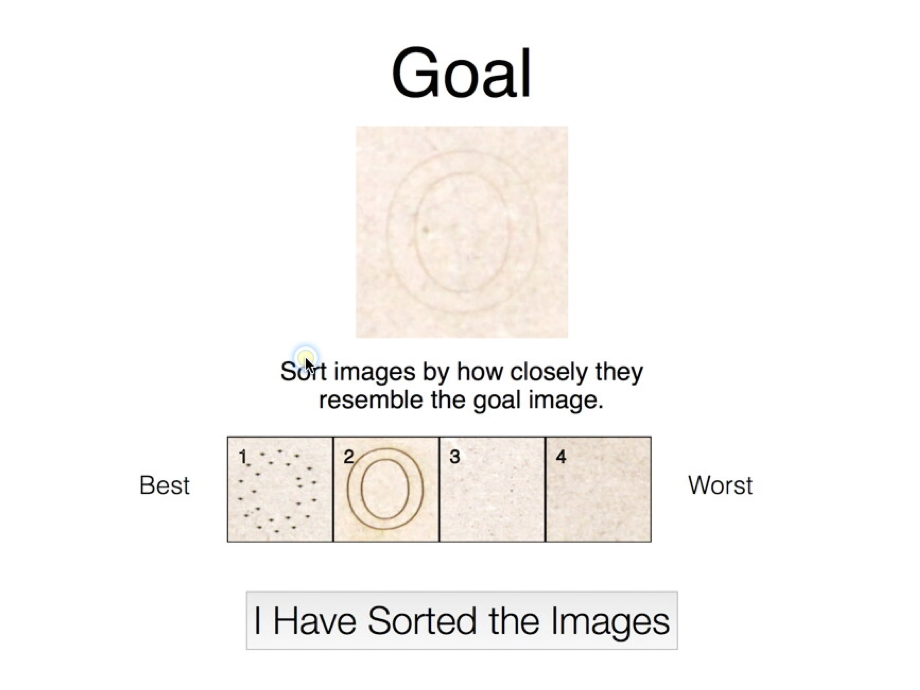
\includegraphics[width=\textwidth]{figures/interface_nm}}
    \caption{Nelder-Mead}\label{fig:interface_nm}
  \end{subfigure}
  \quad
  \begin{subfigure}[b]{0.22\textwidth}
    \fbox{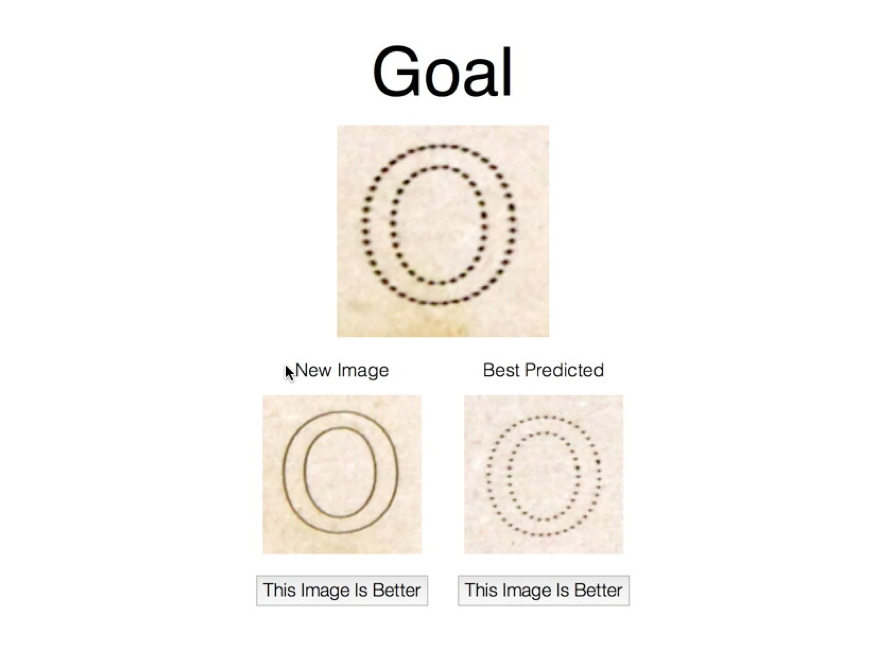
\includegraphics[width=\textwidth]{figures/interface_bo}}
    \caption{Bayesian Optimization}\label{fig:interface_bo}
  \end{subfigure}
  \caption{Interaces.}\label{fig:interfaces}
\end{figure}

\subsection{Nelder-Mead}

At each step, the Nelder-Mead algorithm needs to know which vertex in the simplex is the worst.
In some circumstances, it needs to know which one is the best, and which is second-to-worst.

All of these can be collected at once if a human provides a ranked list from best to worst of the quality of each of the points.
I built an interface to provide rankings to the Nelder-Mead algorithm (see Figure~\ref{fig:interface_nm}).
The output for each of the vertices is shown.
A human ranks each vertex by ordering their output---the images---from best to worst.
This is implemented with an ``insertion sort'' mechanism:
a user moves a vertex to a position in the list, and it displaces all vertexes to the right of it by moving them rightward.

When a user has finished ranking the examples, they click a button reporting they are finished.
The simplex then determines candidate next points (a reflection, expansion, or contraction) and presents these points within the list.
Based on the rank of the generated points, it determines whether to keep the new point or generate a different candidate point.

\subsection{Bayesian Optimization}

Brochu et al.'s variant on Bayesian optimization~\cite{brochu_tutorial_2010} suggests that an optimal point for an unknown cost function can be found by collecting comparison ratings between pairs of points.
In their implementation, a user was shown the best example seen so far, and an examples with the highest expected improvement.
Each ranking would be used to update both the best example seen so far, and the model for choosing a point based on expected improvement.

My interface for Bayesian Optimization is similar to Brochu et al.'s (see Figure~\ref{fig:interface_bo}).
A user is shown the best rated example, and an example that maximizes the expected improvement.
With each rating, both the best rated example and that which maximizes expected imporvement are updated.
The goal is shown between the two examples for a point of reference towards which users work.


\section{Experiment}

I recruited 28 participants on Mechanical Turk.
We accepted workers for whom 95\% of past tasks were approved.
The design was between-subjects.
Each participant was assigned either the Nelder-Mead interface or the Bayesian optimization interface, and one of two goal configurations.
They were shown an image of an engraved `O' produced with the ``goal'' configuration (see Figure~\ref{fig:interfaces}).
They were asked to rank example images based on their closeness to the goal as they attempted to lead the algorithm to the goal.

They completed the activity when they had either submitted 20 rankings, or had marked the goal configuration as the best.
I chose 20 rankings for three reasons.
First, it appeared reasonable from personal testing that participants could achieve an image close to the provided goals with the initial points chosen with that many rankings, with both interfaces.
Second, the Nelder-Mead method seemed to converge to a set of very similar examples before reaching the 20th iteration.
I wanted to avoid participant attrition when they felt like the algorithm was no longer responding to their rankings.
Third, I needed to impose a limit on the number of rankings a participant submitted to let them finish the task an claim their compensation in a reasonable amount of time.

Participants were not allowed to end their participation by just reporting that they had reached the goal configuration---%
the goal configuration actually had to be presented to them by the algorithm, and they had to report it as the best one.
This was to prevent participants from falsely reporting having achieved the goal in order to claim early compensation.
Each participants were paid \$1.00 for this HIT\@.

In a follow-up questionnaire, participants were rated their agreement with six statements on a 5-point Likert scale:
\begin{itemize}[noitemsep]
\item I trusted that the algorithm would show me better images in each round.
\item I don't understand why the algorithm chose the examples it did.
\item The algorithm got stuck.  It kept picking images that weren't what I wanted.
\item The last image I marked as best was very similar to the goal image.
\item The algorithm's guesses got better over time.
\item The algorithm made random choices about what to show me.
\end{itemize}
These statements were chosen to capture participants' feelings of the algorithms randomness, trustworthiness and success in attaining a goal, and change in behavior over time.
They were based on Hoffman's recommended metrics for evaluating robot fluency~\cite{hoffman_evaluating_2013}.
Although I was not evaluating fluency, I was interested in assessing perceptions of an algorithm's contribution, trust, and satisfaction, for which Hoffman provided initial ideas.
The order of the questions was not randomized, but it should be in future versions of this study.


\section{Results}

When discussing results, I refer to conditions with acronyms NM for Nelder-Mead, and BO for Bayesian optimization.

First, which algorithm was better able to help participants achieve their goals?
In the BO condition, participants' best-rated configurations were much closer to their goal than in the NM condition (see Figure~\ref{fig:bestfits}),
By looking at longitudinal data (Figure~\ref{fig:best_distances}), it appears that by iteration 10, participants in the BO condition were, in general, closer to their goal than participants in the NM condition.

\begin{figure}
  \centering
  \begin{subfigure}[b]{0.23\textwidth}
    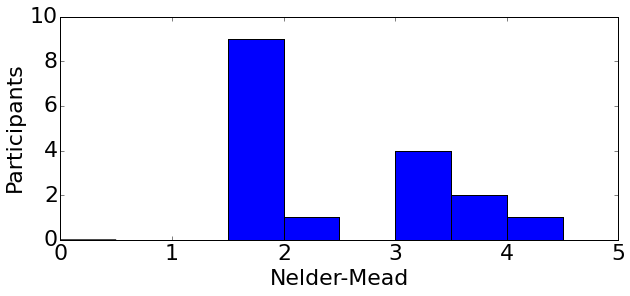
\includegraphics[width=\textwidth]{figures/bestfits_nm}
  \end{subfigure}
  \begin{subfigure}[b]{0.23\textwidth}
    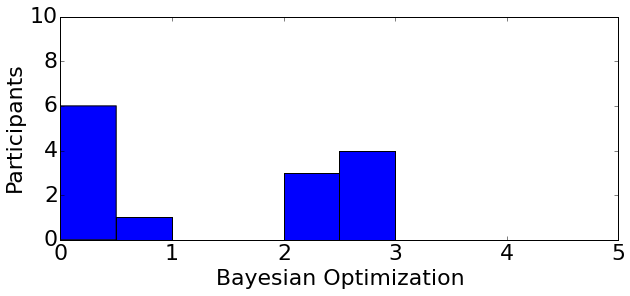
\includegraphics[width=\textwidth]{figures/bestfits_bo}
  \end{subfigure}
  \caption{Distance of a participant's best-rated point and the goal configuration for each algorithm.}\label{fig:bestfits}
\end{figure}

\begin{figure}
\centering
  \begin{subfigure}[b]{0.48\textwidth}
    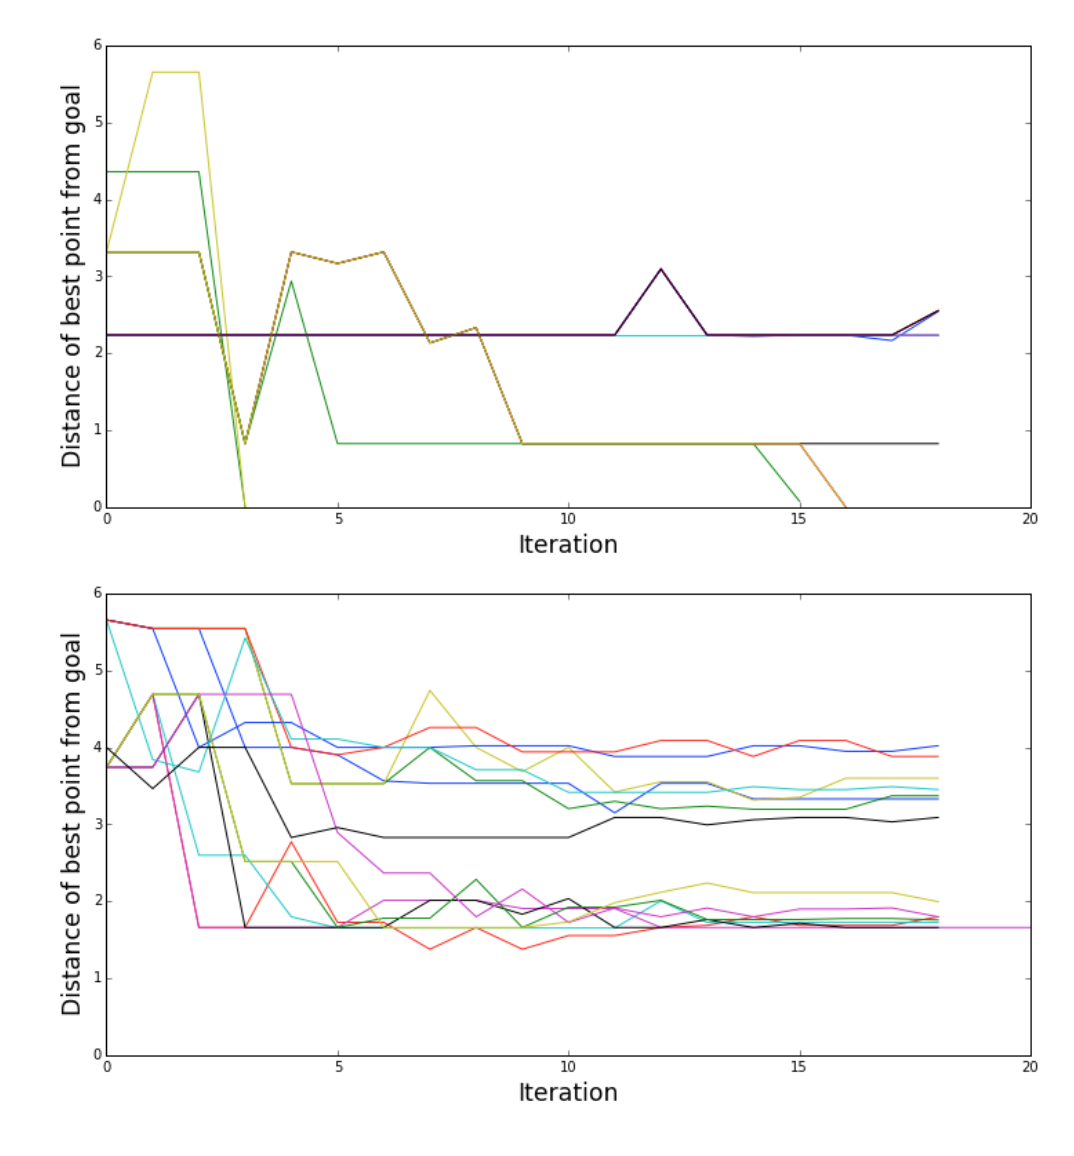
\includegraphics[width=\textwidth]{figures/best_distances}
    \caption{%
      With each successive ranking, the distance of a participant's best-rated point from the goal configuration.
    }\label{fig:best_distances}
  \end{subfigure}
  \begin{subfigure}[b]{0.48\textwidth}
    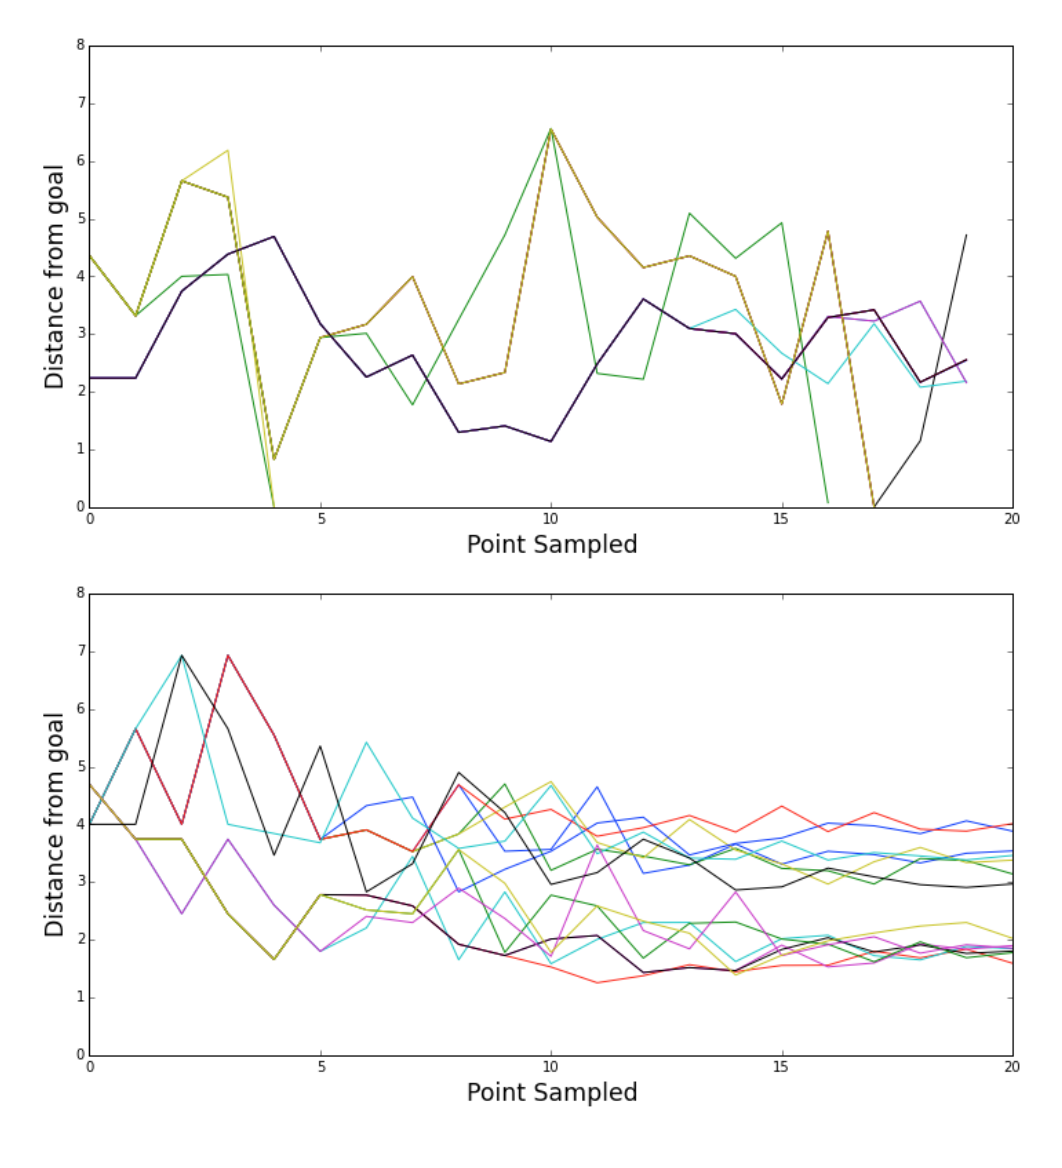
\includegraphics[width=\textwidth]{figures/point_distances}
    \caption{%
      The distance of each new point an algorithm proposes from the goal configuration.
    }\label{fig:point_distances}
  \end{subfigure}
  \caption{%
    Distances of best-rated or proposed points from goal configurations.
    Each line represents one participant working with one algorithm.
    For each pair of plots,
    Bayesian optimization is shown on the top, and 
    Nelder-Mead on the bottom.
  }
\end{figure}

When we observe the paths of points provided by each of the algorithms, we see differing approaches in the points proposed.
In its current form, participants using BO clearly covered more of the parameter space (see Figure~\ref{fig:coverage}).
For NM, it appears that vertices were gradually pulled in toward some center where the simplex converged.
In fact, this motion looks mostly planar.
BO, in comparison, appears almost like random sampling.
This may be in part due to our particular choice of kernel $\sigma$ and noise standard deviation $\sigma_{noise}$.

\begin{figure}
  \centering
  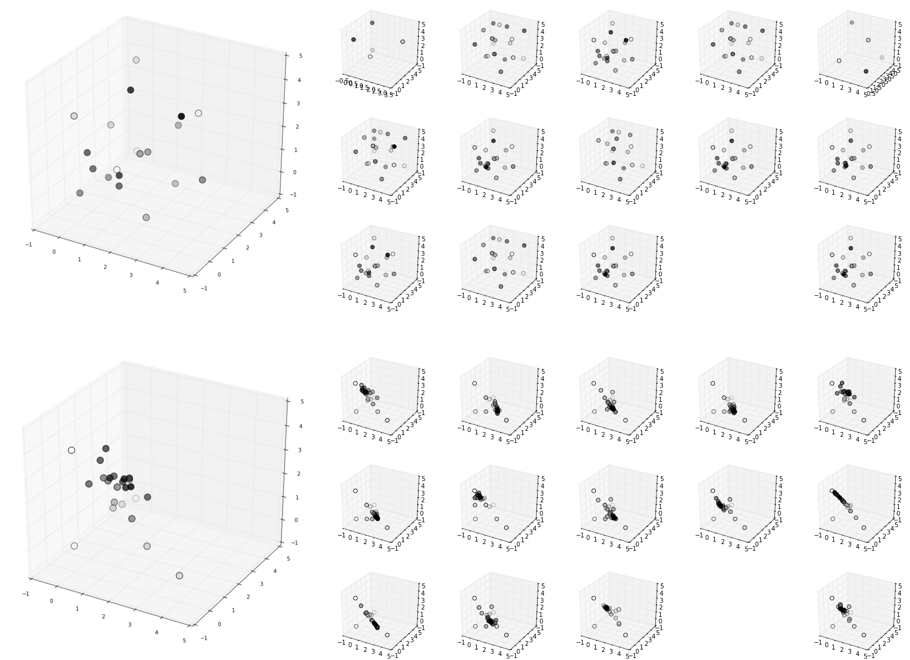
\includegraphics[width=0.48\textwidth]{figures/scatters}
  \caption{%
    The points that each algorithm proposed.
    The first three rows show participants using Bayesian optimization.
    The bottom three rows show participants using Nelder-Mead.
    An enlarged exemplar for each method is shown to the left of the small multiples.
    The first point an algorithm proposes is shown in white;
    Each new point is more grey than the last, until the final point is black.
  }\label{fig:coverage}
\end{figure}

When we consider the distance of each of the proposed points from the goal, we see why BO outperformed NM\@.
Figure~\ref{fig:point_distances} shows how the distance of the latest point proposed changes over time for each algorithm.
After about the tenth point sampled, it appears as if Nelder-Mead no longer suggests new examples radically farther from the goal.
This may be an indication of NM prematurely converging to a local maximum.
BO, on the other hand, continues to suggest points both near and far from the goal, and does not appear to converge at all.

Participants perceived these differences in how the algorithms worked (see Figure~\ref{fig:feedback}).
Those in the BO condition were more likely to report that the algorithm's choice of points seemed random.
But these participants were also more likely to claim that the point they marked as the best was very close to the goal.
Participants working with NM more often reported that the algorithm seemed to improve over time.
However, it also seemed more likely to get stuck.

\begin{figure}
  \centering
  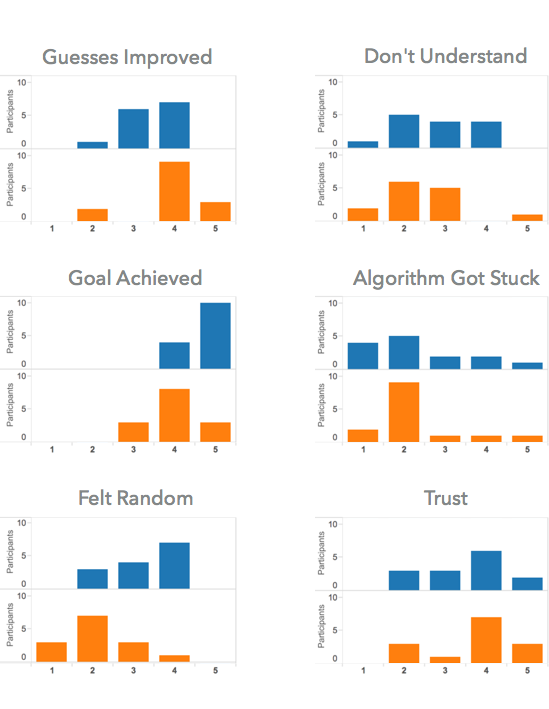
\includegraphics[width=0.4\textwidth]{figures/feedback}
  \caption{%
    Participant responses to questions about their perception of each algorithm.
    Blue bars show participants in the Bayesian optimization condition.
    Orange bars show participants in the Nelder-Mead condition.
  }\label{fig:feedback}
\end{figure}

\subsection{Limitations}

Participants were forced to stop after reporting 20 rankings to the algorithm.
I expect that that the Bayesian optimization algorithm would have seemed less random over time.
The choice of hyperparameters for NM and BO might impact user perceptions of randomness and the best point a participant finds after 20 rankings.
Before drawing any conclusions about these algorithms, a wider, systematically-determined range of hyperparameters must be tested.

Many of the participants in the BO condition achieved exactly the goal after only a few rankings (see Figure~\ref{fig:coverage}).
It's likely that one of the goals was ``just right'' for participants in the BO condition to discover precisely the right condition after only a few comparisons.
This suggests that this one goal was better suited to BO than NM for these tests, and weakens any potential claims about inherent strengths of BO at finding configurations close to the goal.
To counter this side effect and improve generalizability, a larger number of goal images should be tested.
Better yet, goal images could be randomly selected from the domain of the input space.


\section{A Preliminary Lab Study}

Before the experiment above, I ran an in-lab study with three participants.
As the motivating domain for this paper is fabrication, I sought to compare one optimization technique---Nelder-Mead---with a baseline interface for discovering the right engraving settings.
In particular, participants would view and rank physical, laser-engraved examples.

Participants used either the Nelder-Mead interface or a slider-based interface to guide the laser cutter to choosing engraving parameters.
The slider-based interface was a near-direct copy of the software user interface for the Universal Laser Systems VersaLaser 3.50, a modern laser cutter.
Just like in the original interface, there was no indication of how these parameters would affect how the laser engraved, or how the result would appear.
The experimenter provided no description of the parameters.

Similarly to the MTurk experiment, participants were provided with a goal---
a physical 2cm$\times$2cm tile with an engraved `O'.
This was cut on a soft particle wood 3mm thick.
With the slider-based interface, participants moved sliders to change the values of power, speed and PPI to alter the engraving appearance.
They were given pen and paper to take notes as they worked to understand how these parameters affected the appearance.
With the Nelder-Mead interface, similar to above, participants ordered engravings from left to right based on their closeness to the goal.
Unlike the MTurk study, participants in the lab could actually do this ranking with the physical workpieces.
After ordering them on the table, they entered their ranking into the software interface.
The experimenter fed the suggested parameters from the algorithm into the laser cutter to engrave each new example.

While participants' screens were recorded and all examples saved, I have yet to process this data.
My intuitions are that participants were able to try out more examples with less time in-between with the Nelder-Mead interface than with the baseline interface.
However, participants were also frustrated, confused, or skeptical when the Nelder-Mead interface converged on an maximum that was not their goal.
Feedback from this study also inspired the author to improve the ranking interface to support insertion sort-based ranking mechanics, to avoid showing a reflection, expansions and contraction all at once, and to improve bugs that were uncovered.


%\section{Discussion}

\subsection{Future Work}

I worked to produce expression mechanisms for the algorithms that closely matched the input to each of the algorithm and would be rapid for users to produce.
However, it's not clear that these are the best expression mechanisms.

Furthermore, additional work would need to be done to understand how rankings and comparisons could be implemented physically for users working with a fabrication machine.

Scale this up to a larger input space.


\section{Conclusion}

People frequently have to work with machines to achieve some subjective goal with parameters they do not understand.
This paper compares two algorithms to help humans achieve such goals by systematically exploring parameter spaces.
While the Nelder-Mead optimization method appears less random to users than Bayesian optimization, the latter appears less likely to prematurely converge.
Future work should address three issues.
First, it should provide a systematic review of algorithms equipped to solve this problem and a comparison of human perceptions of these methods.
Second, it should explore a wider range of mechanisms for expressing rankings, beyond just pairs and sorted lists.
Third, it should do this in a domain-independent way, beyond just fabrication machines.


\section{Acknowledgments}

Thanks to Jessica Hamrick for introducing me to psiTurk tool and helping me get access to it.
Thanks also Anca Dragan, Chelsea Finn, Ben Caulfield and Manuel Sabin for their help choosing and tweaking the algorithms for this project.

% Balancing columns in a ref list is a bit of a pain because you
% either use a hack like flushend or balance, or manually insert
% a column break.  http://www.tex.ac.uk/cgi-bin/texfaq2html?label=balance
% multicols doesn't work because we're already in two-column mode,
% and flushend isn't awesome, so I choose balance.  See this
% for more info: http://cs.brown.edu/system/software/latex/doc/balance.pdf
%
% Note that in a perfect world balance wants to be in the first
% column of the last page.
%
% If balance doesn't work for you, you can remove that and
% hard-code a column break into the bbl file right before you
% submit:
%
% http://stackoverflow.com/questions/2149854/how-to-manually-equalize-columns-
% in-an-ieee-paper-if-using-bibtex
%
% Or, just remove \balance and give up on balancing the last page.
%
\balance{}

% REFERENCES FORMAT
% References must be the same font size as other body text.
\bibliographystyle{acm}
\bibliography{references}

\end{document}

%%% Local Variables:
%%% mode: latex
%%% TeX-master: t
%%% End:
